\chapter{Inventario / Catálogo}
\label{mod:07-inventario-catalogo}

\section{Propósito}
\label{sec:07-proposito}

Administra el catálogo de productos de la óptica (armazones, accesorios y el catálogo óptico legado de cristales) y controla el stock por sucursal mediante un registro auditable de movimientos, en vez de un campo mutable. Incluye trazabilidad de lotes con vencimiento, conteos físicos periódicos con ajuste, y el catálogo de clasificaciones ópticas (\code{TipoLente}, \code{Tratamiento}) que consume el módulo de Ventas (Capítulo~\ref{mod:08-ventas}) para el flujo ``a pedido''.

\section{Entidades principales}
\label{sec:07-entidades}

\begin{longtable}{p{3.4cm}p{10.2cm}}
\caption{Entidades principales del módulo de Inventario/Catálogo.}
\label{tab:07-entidades}\\
\toprule
\textbf{Entidad} & \textbf{Rol} \\
\midrule
\endfirsthead
\toprule
\textbf{Entidad} & \textbf{Rol} \\
\midrule
\endhead
\bottomrule
\endfoot
\code{Producto} & Ítem de catálogo con stock (armazones, accesorios); \code{PrecioVenta} siempre derivado \\
\code{CategoriaProducto} & Categoría con \code{Margen} (define el precio de venta) y \code{Tipo} (Genérico/Armazón/\textbf{Cristal obsoleto}) \\
\code{Marca} / \code{Modelo} & Catálogo jerárquico de marca $\rightarrow$ modelo \\
\code{Producto}\allowbreak \code{Stock}\allowbreak \code{Config} & Mín/máx de stock, 1:1 con \code{Producto}, \textbf{global} (no por sucursal) \\
\code{MovimientoStock} & Entrada/Salida con \code{Estado} Pendiente/Aprobado/Rechazado --- única fuente del stock real \\
\code{MotivoMovimiento} & Catálogo de motivos, filtra por tipo de movimiento \\
\code{StockLote} & Trazabilidad de lotes con \code{FechaVencimiento}, originados en una recepción \\
\code{ConteoInventario} / \code{Conteo}\allowbreak \code{Inventario}\allowbreak \code{Linea} & Conteo físico periódico con diferencia sistema-vs-físico \\
\code{StockActualView} & Entidad de solo lectura sobre la vista SQL \code{vw_stock_actual} \\
\code{TipoLente} & Diseño de lente (monofocal/bifocal/progresivo/ocupacional) con \code{PrecioBase} --- usado por Ventas/Laboratorio \\
\code{Tratamiento} & Tratamiento óptico con precio (antirreflejo, fotocromático, etc.) --- N:N con \code{TrabajoPedido} \\
\code{Transferencia}\allowbreak \code{Stock} / \code{Item} & Transferencia entre sucursales --- detalle completo en el Capítulo~\ref{mod:15-sucursales} \\
\end{longtable}

Ver diagrama ER completo en el Capítulo~\ref{sec:modelo-datos}, Figura~\ref{fig:er-inventario-stock}. Los servicios (exámenes con tarifa por profesional) se documentan en el Capítulo~\ref{mod:08-ventas}.

\section{Reglas de negocio clave}
\label{sec:07-reglas}

\begin{itemize}
  \item \textbf{El stock no es un campo, se deriva de movimientos aprobados.} Ver \hyperref[adr:0002]{ADR 0002}. \code{vw_stock_actual} agrupa por producto más sucursal sumando Entrada (+) / Salida (--) sobre los movimientos en estado \code{Aprobado} (la vista compara contra el ordinal del enum, no contra una cadena).
  \item \textbf{\code{PrecioVenta} siempre derivado, nunca manual.} \code{PrecioCosto} $\times$ (1 + \code{CategoriaProducto.}\allowbreak \code{Margen}/100), centralizado en \code{Producto.}\allowbreak \code{AplicarCosto}. Ver \hyperref[adr:0004]{ADR 0004}. Cambiar el margen de una categoría recalcula todos sus productos.
  \item \textbf{El catálogo óptico de cristales está obsoleto.} \code{CategoriaProducto.Tipo = Cristal} ya no se ofrece al dar de alta categorías (se conserva solo por compatibilidad de datos existentes). El cristal a pedido se especifica en el \code{TrabajoPedido} del módulo Ventas, no como \code{Producto}. Ver \hyperref[adr:0007]{ADR 0007} --- \textbf{no confundir con \code{TipoLente}/\code{Tratamiento}} de esta lista, que siguen vigentes (son la especificación del cristal, no un producto con stock).
  \item \textbf{\code{Producto}\allowbreak \code{Stock}\allowbreak \code{Config} es global, no por sucursal} --- decisión explícita para no invalidar la relación 1:1 durante la migración multi-sucursal.
  \item \textbf{Crear un conteo de inventario exige solo \code{ver_inventario}}; únicamente \emph{gestionar} (aprobar/rechazar, lo que ajusta el stock) exige \code{gestionar_}\allowbreak \code{inventario} --- asimetría real del código, no error de este documento.
  \item \textbf{Los estados de inventario son enums, igual que en el resto del sistema:} \code{MovimientoStock.}\allowbreak \code{Estado}/\code{.Tipo}, \code{ConteoInventario.}\allowbreak \code{Estado}, \code{TransferenciaStock.}\allowbreak \code{Estado} y \code{MotivoMovimiento.}\allowbreak \code{Tipo} son enums C\# persistidos como \code{int}, con la misma convención que \code{Venta}/\code{TrabajoPedido}/\code{Egreso}. Ver el Capítulo~\ref{sec:modelo-datos}, Cuadro~\ref{tab:enums}.
\end{itemize}

\section{Endpoints}
\label{sec:07-endpoints}

Detalle completo en el Apéndice de Referencia de API, § Catálogo/Inventario. Resumen:

\begin{longtable}{p{4cm}p{3cm}p{5.6cm}}
\caption{Controllers del módulo de Inventario/Catálogo.}
\label{tab:07-endpoints}\\
\toprule
\textbf{Controller} & \textbf{Ruta base} & \textbf{Cubre} \\
\midrule
\endfirsthead
\toprule
\textbf{Controller} & \textbf{Ruta base} & \textbf{Cubre} \\
\midrule
\endhead
\bottomrule
\endfoot
\code{Productos}\allowbreak \code{Controller} & \code{/api/productos} & CRUD de productos, movimientos de stock, stock-config, imagen, y sub-recursos \code{categorias} (\code{CategoriaProducto}) \\
\code{MarcasController} & \code{/api/marcas} & CRUD de marcas y sub-recurso \code{modelos} (\code{Modelo}) \\
\code{Tipo}\allowbreak \code{Lentes}\allowbreak \code{Controller} & \code{/api/}\allowbreak \code{tipos-lente} & CRUD de diseños de lente \\
\code{Tratamientos}\allowbreak \code{Controller} & \code{/api/}\allowbreak \code{tratamientos} & CRUD de tratamientos \\
\code{Motivos}\allowbreak \code{Movimiento}\allowbreak \code{Controller} & \code{/}\allowbreak \code{api/}\allowbreak \code{motivos-}\allowbreak \code{movimiento} & CRUD de motivos, filtrable por tipo \\
\code{Stock}\allowbreak \code{Lotes}\allowbreak \code{Controller} & \code{/api/stock/}\allowbreak \code{lotes} & Lotes con vencimiento más conteos físicos (crear/listar/gestionar) \\
\code{Ubicaciones}\allowbreak \code{Controller} & \code{/api/}\allowbreak \code{ubicaciones} & \code{Departamento}/\code{Ciudad} --- catálogo geográfico compartido con Sucursal/Proveedor, no exclusivo de este módulo \\
\end{longtable}

\section{Flujo típico}
\label{sec:07-flujo}

\textbf{Movimiento de stock con aprobación:}

\begin{figure}[htbp]
\centering
\begin{tikzpicture}[node distance=1.4cm]
  \node[actor] (u) at (0,0) {Usuario\\\footnotesize (\code{gestionar_}\allowbreak \code{inventario})};
  \node[actor] (api) at (4,0) {ProductosController};
  \node[actor] (svc) at (8.5,0) {ProductoService /\\MovimientoStockService};
  \node[actor] (db) at (13,0) {PostgreSQL};

  \draw[lineavida] (u.south) -- ++(0,-8.5);
  \draw[lineavida] (api.south) -- ++(0,-8.5);
  \draw[lineavida] (svc.south) -- ++(0,-8.5);
  \draw[lineavida] (db.south) -- ++(0,-8.5);

  \draw[mensaje] ($(u.south)+(0,-1)$) -- node[above,font=\scriptsize]{POST /api/productos/\{id\}/movimientos} ($(api.south)+(0,-1)$);
  \draw[mensaje] ($(api.south)+(0,-2)$) -- node[above,font=\scriptsize]{CreateMovimientoStockRequest} ($(svc.south)+(0,-2)$);
  \draw[mensaje] ($(svc.south)+(0,-3)$) -- node[above,font=\scriptsize]{INSERT MovimientoStock (Estado=Pendiente)} ($(db.south)+(0,-3)$);
  \node[font=\scriptsize\itshape, align=center] at (10.75,-3.9) {vw\_stock\_actual sin cambios\\(solo cuenta Aprobado)};

  \draw[mensaje] ($(u.south)+(0,-5.2)$) -- node[above,font=\scriptsize]{PATCH .../movimientos/\{id\}/estado} ($(api.south)+(0,-5.2)$);
  \draw[mensaje] ($(api.south)+(0,-6.2)$) -- node[above,font=\scriptsize]{AprobarRechazarMovimientoRequest} ($(svc.south)+(0,-6.2)$);
  \draw[mensaje] ($(svc.south)+(0,-7.2)$) -- node[above,font=\scriptsize]{UPDATE MovimientoStock SET Estado=Aprobado} ($(db.south)+(0,-7.2)$);
  \node[font=\scriptsize\itshape, align=center] at (10.75,-8.1) {vw\_stock\_actual recalcula\\al leer (suma el movimiento)};
\end{tikzpicture}
\caption{Movimiento de stock: alta en \texttt{Pendiente} y aprobación posterior, que recién ahí impacta \texttt{vw\_stock\_actual}.}
\label{fig:seq-movimiento-stock}
\end{figure}

\textbf{Conteo físico:} cualquier usuario con \code{ver_inventario} registra un \code{ConteoInventario} con sus \code{Conteo}\allowbreak \code{Inventario}\allowbreak \code{Linea} (cantidad física por producto); el sistema calcula \code{Diferencia} contra \code{vw_stock_actual}. Solo un usuario con \code{gestionar_}\allowbreak \code{inventario} puede aprobar el conteo --- la aprobación genera los \code{MovimientoStock} de ajuste necesarios para que el stock del sistema coincida con lo contado.

\section{Vistas de frontend}
\label{sec:07-frontend}

\code{ProductosView.vue}, \code{CategoriasProductoView.}\allowbreak \code{vue}, \code{MarcasView.vue}, \code{ModelosView.vue}, \code{TipoLentesView.}\allowbreak \code{vue}, \code{TratamientosView.}\allowbreak \code{vue}, \code{StockView.vue}, \code{MovimientosView.}\allowbreak \code{vue}, \code{MovimientoFormView.}\allowbreak \code{vue}, \code{MotivosMovimientoView.}\allowbreak \code{vue}, \code{ConteoFormView.}\allowbreak \code{vue}, \code{ConteoRevisarView.}\allowbreak \code{vue}, \code{ConteoAprobacionView.}\allowbreak \code{vue}, \code{ConteoAprobacion}\allowbreak \code{PendientesView.}\allowbreak \code{vue} (todas en \code{SIGA-Web/}\allowbreak \code{src/}\allowbreak \code{views/}).

\section{Interfaz}
\label{sec:07-interfaz}

\begin{figure}[htbp]
\centering
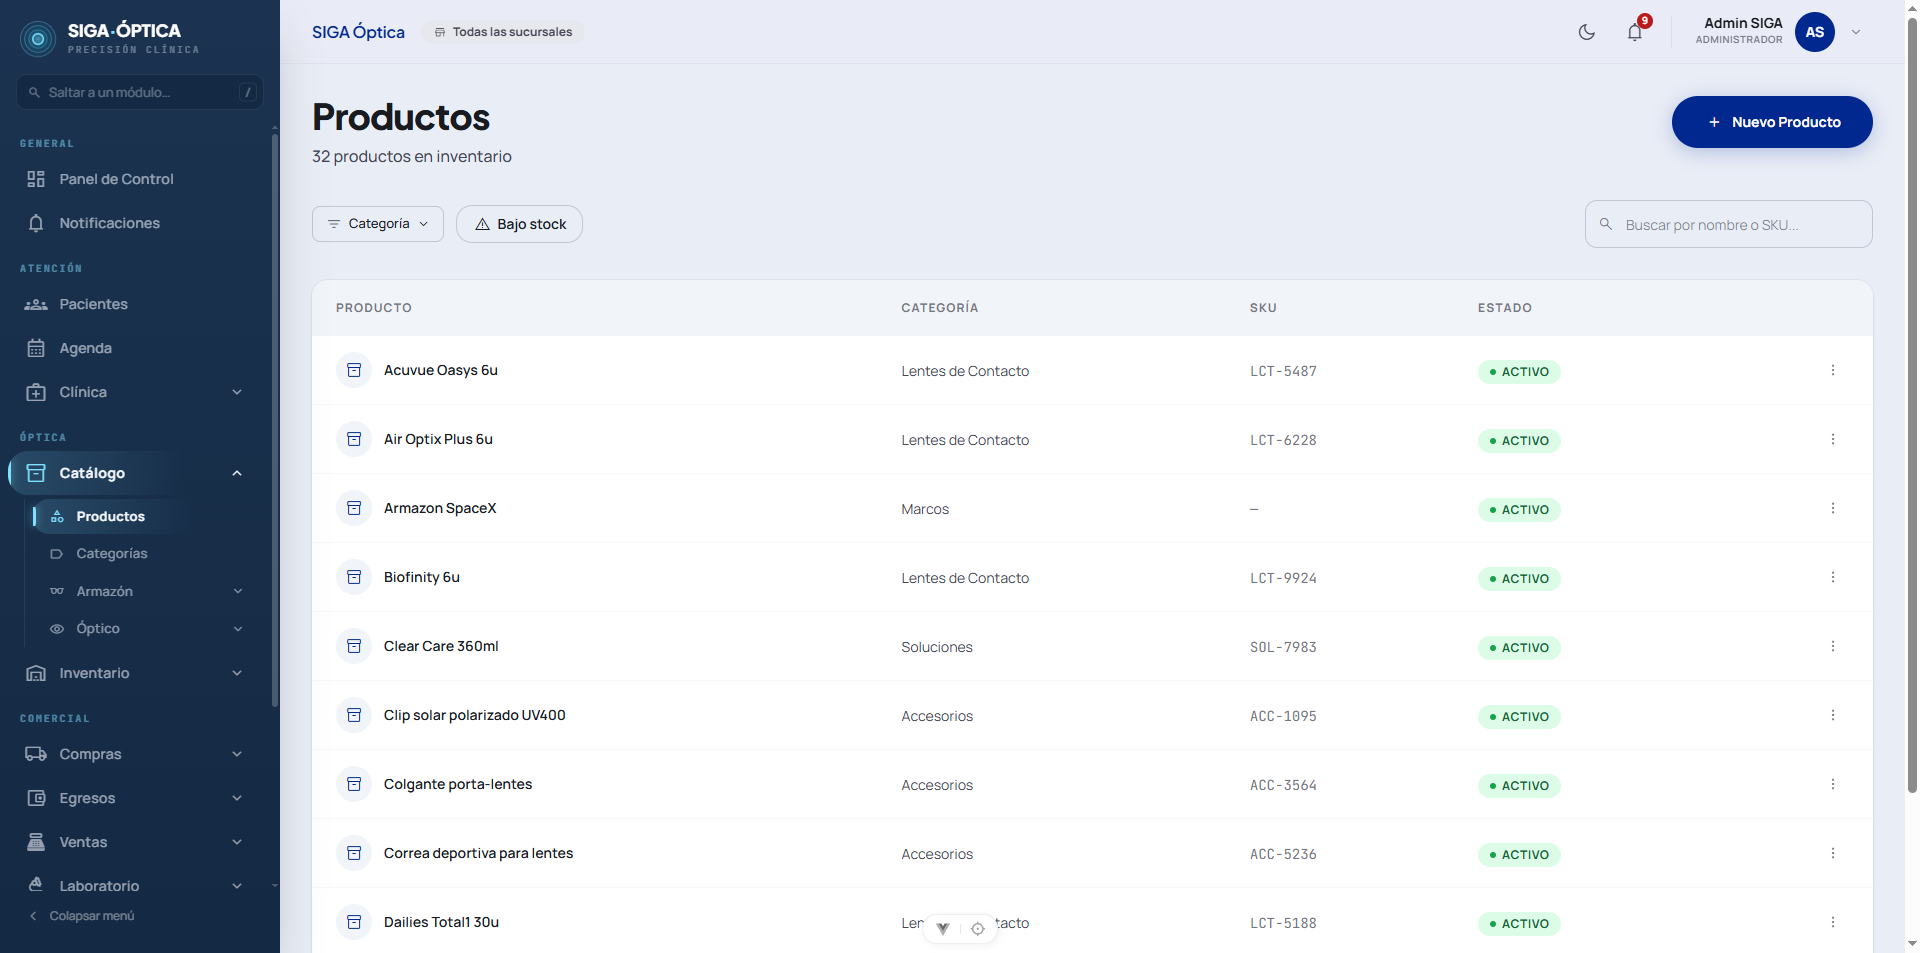
\includegraphics[width=0.95\textwidth]{imagenes/mod07-inventario-productos.png}
\caption{Catálogo de productos, con categoría, SKU y estado de cada uno.}
\label{fig:mod07-inventario}
\end{figure}

\section{Estado}
\label{sec:07-estado}

\Implementado\ y en uso. Dos decisiones de diseño explícitas que conviene tener presentes:
\begin{itemize}
  \item \code{Producto}\allowbreak \code{Stock}\allowbreak \code{Config} define los niveles mínimo y máximo de forma global, no por sucursal.
  \item Las categorías con \code{Tipo = Cristal} y los productos asociados a ellas quedan como datos legado: siguen existiendo en la base por trazabilidad histórica, pero no se ofrecen en altas nuevas (ver \hyperref[adr:0007]{ADR 0007}).
\end{itemize}
